% =============================================================================
% Section 1.1: Motivation and Justification
% =============================================================================

\section{Motivation and Justification}
\label{sec:motivation}

\subsection{The Post-COVID E-Learning Market}
\label{subsec:post-covid-market}

The global e-learning industry has undergone a structural and likely permanent transformation since the COVID-19 pandemic forced universities, training providers, and enterprises to deliver instruction remotely at unprecedented scale. What was previously treated as a supplementary channel---useful for corporate compliance modules or distance-learning electives---has become a primary delivery mechanism for degree programmes, professional certification, and independent creator economies. Industry analyses value the global e-learning market at approximately \$250--400~billion in the mid-2020s, with compound annual growth rates consistently projected in the double digits through the end of the decade. Growth drivers include corporate upskilling mandates, higher-education digitisation, mobile-first learners in emerging markets, and the proliferation of creator-led course businesses.

Leading commercial platforms illustrate the scale that modern backends must support. \textbf{Udemy} reports tens of millions of registered learners and hundreds of millions of course enrolments cumulatively; peak traffic during promotional events stresses payment, entitlement, and content-delivery subsystems simultaneously. \textbf{Coursera} partners with universities worldwide and must reconcile academic calendars, verified credentials, and enterprise B2B contracts within shared infrastructure. \textbf{LinkedIn Learning}, \textbf{edX}, and regional platforms such as \textbf{Udacity} and \textbf{Pluralsight} similarly combine video libraries, assessments, progress tracking, and monetisation in unified user experiences. Although NexaLearn is scoped as a graduation project rather than a hyperscale production deployment, it is deliberately engineered against the \textit{functional} and \textit{architectural} expectations these platforms establish: stateless horizontally scalable API tiers, durable workflow orchestration, secure payment settlement, entitlement-aware media delivery, and analytics that inform instructor and operator decisions.

The post-COVID era also normalised hybrid instructional models in which asynchronous video modules coexist with synchronous sessions, formative AI-generated quizzes supplement summative exams, and discussion forums extend classroom dialogue. Backend systems must therefore support not only CRUD operations on course catalogues, but long-running asynchronous pipelines (transcoding, transcription, question generation), fine-grained authorisation (instructor, student, admin, teaching assistant roles), and cross-module eventual consistency without sacrificing user-visible correctness.

\subsection{Fragmentation of Existing Open-Source and Template Solutions}
\label{subsec:fragmentation}

Despite market maturity, the software engineering community lacks a cohesive, open, and pedagogically transparent backend that unifies the full breadth of e-learning concerns within a single architecturally disciplined codebase. The gap manifests in three distinct categories of alternative, each insufficient as a holistic reference.

\textbf{Commercial closed platforms.} Udemy, Coursera, Teachable, Thinkific, and Kajabi deliver polished end-user experiences but expose only narrow public APIs. Internal service boundaries, saga implementations, event schemas, and consistency models remain trade secrets. Independent engineering teams cannot inspect how enrollment activation is coupled to payment webhooks, how video DRM integrates with progress checkpoints, or how AI-generated assessments are validated before publication. Vendor lock-in and revenue-sharing models further discourage universities and startups seeking data sovereignty.

\textbf{Legacy open-source LMS platforms.} Moodle, Sakai, and Canvas (open-core) evolved over decades as plugin-oriented PHP or Java monoliths. They prioritise feature breadth---forums, gradebooks, SCORM players, attendance plugins---over modular domain clarity. Cross-plugin coupling, shared global state, and inconsistent API layers make it difficult to extract modern patterns such as bounded contexts, transactional outboxes, or typed domain events. Moodle's architecture, while battle-tested at institutional scale, reflects design decisions from an era before widespread REST microservices, TypeScript type safety, and cloud-native video pipelines.

\textbf{Specialised micro-templates and generic boilerplates.} The NestJS ecosystem offers numerous starter repositories providing JWT authentication, Prisma CRUD, and Docker Compose scaffolding. Separate commercial services address individual verticals: Stripe for payments, Mux or Cloudflare Stream for video, Algolia for search, SendGrid for email. None of these templates demonstrate how fifteen or more bounded contexts should collaborate under shared transactional guarantees, nor do they implement e-learning-specific state machines (pending enrollment awaiting payment, video asset awaiting transcoding, quiz attempt awaiting async grading). Developers assembling these pieces ad hoc frequently produce systems that \textit{appear} functional in demos but fail under duplicate webhook delivery, concurrent course edits, or partial pipeline failures.

Table~\ref{tab:platform-comparison-intro} summarises the principal limitation motivating NexaLearn: no widely available open reference spans authentication, structured course aggregates, payment-backed enrollment, Mux-integrated media, Whisper/LLM AI pipelines, assessment, social learning, certificates, search, streaks, notifications, and instructor analytics within one DDD-governed NestJS codebase.

\begin{table}[H]
  \centering
  \caption{High-Level Comparison of Platform Categories Relevant to NexaLearn Motivation}
  \label{tab:platform-comparison-intro}
  \small
  \begin{tabular}{@{}p{2.8cm} p{3.2cm} p{3.5cm} p{3.8cm}@{}}
    \toprule
    \textbf{Category} & \textbf{Representative Examples} & \textbf{Primary Strengths} & \textbf{Gap NexaLearn Addresses} \\
    \midrule
    Commercial SaaS &
    Udemy, Coursera, Teachable &
    Polished UX, scale, content marketplace &
    No source access; opaque architecture; vendor lock-in \\
    \addlinespace
    Legacy OSS LMS &
    Moodle, Open edX, Sakai &
    Institutional adoption; rich plugin ecosystems &
    Monolithic plugin sprawl; dated stacks; weak DDD \\
    \addlinespace
    Generic NestJS starters &
    Community boilerplates &
    Fast bootstrap; JWT + ORM patterns &
    No e-learning domain; no outbox; no Stripe/Mux/AI \\
    \addlinespace
    Vertical SaaS APIs &
    Stripe, Mux, OpenAI &
    Best-in-class single concern &
    No unified domain model or cross-context reliability \\
    \bottomrule
  \end{tabular}
\end{table}

\subsection{Architectural Challenges Facing E-Learning Backend Developers}
\label{subsec:architectural-challenges}

Developers who attempt to build e-learning platforms from scratch encounter recurring architectural challenges that introductory web development curricula rarely address. These challenges form the technical core of NexaLearn's motivation.

\textbf{Cross-bounded-context workflow orchestration.} A representative student journey traverses Search (discovery), Enrollment (intent), Payments (settlement), Courses/Media (consumption), Progress (checkpointing), Assessment (validation), Certificates (credential), Reviews (feedback), Notifications (engagement), and Streak (retention). Each step is owned by a distinct module with its own aggregates and invariants. Naive implementations invoke synchronous service calls across module boundaries, creating availability cascades and tight coupling. Event-driven designs alleviate synchronous coupling but introduce delivery semantics questions: what happens if the notification dispatcher fails after enrollment activates?

\textbf{Eventual consistency and external callbacks.} Video platforms emit webhooks when uploads complete or renditions become playable; Stripe notifies applications of \texttt{payment\_intent.succeeded} and \texttt{charge.refunded}; AI workers callback with transcription segments or generated question banks minutes to hours later. Network retries cause duplicate deliveries; maintenance windows cause delayed out-of-order arrivals. Without idempotent handlers backed by persistent idempotency keys or outbox deduplication, systems exhibit double enrollment activation, orphaned Mux assets detached from lessons, or students charged without course access---failures that erode trust and create support burden.

\textbf{Concurrency and aggregate integrity.} Instructors reorder lessons while students mark progress; admins publish course revisions while enrollment counts feed analytics dashboards. Lost updates on course structures, duplicate quiz attempts, and race conditions on seat-limited offerings require optimistic or pessimistic concurrency strategies encoded at the domain layer, not patched ad hoc in controllers.

\textbf{Security and compliance surface area.} Authentication must resist credential stuffing (rate limiting), token theft (refresh rotation with reuse detection), and privilege escalation (RBAC with instructor-scoped analytics). Payment endpoints must verify webhook signatures. AI pipeline callbacks must authenticate via HMAC to prevent forged quiz injection. Audit trails must record administrative actions without storing secrets or raw payment instrument data.

\subsection{The AI Imperative in Modern E-Learning}
\label{subsec:ai-imperative}

A further motivation distinct from pre-2020 LMS development is the rapid integration of artificial intelligence into educational workflows. Learners expect searchable transcripts of video lectures; instructors seek automated generation of formative multiple-choice and short-answer questions aligned with lesson content; platform operators explore async grading assistance for open-ended responses to scale human review. These capabilities are not cosmetic feature flags---they imply dedicated pipeline orchestration, job state tracking, cost-aware retry policies, content moderation boundaries, and privacy controls over copyrighted or personally identifiable material submitted to third-party models.

Speech-to-text models such as \textbf{OpenAI Whisper} produce transcripts that feed retrieval and accessibility features. Large language models (LLMs) synthesise question banks when prompted with transcript segments and instructor constraints (difficulty, count, question types). Such pipelines are inherently \textit{asynchronous} and \textit{non-deterministic}: failures, partial results, and model revisions must be handled gracefully without corrupting published assessment entities. Treating AI as a bolt-on script rather than a first-class \textbf{AI Pipeline bounded context} leads to duplicated callback endpoints, inconsistent correlation identifiers, and security gaps when unsigned webhook payloads mutate production quiz data.

NexaLearn addresses this imperative by modelling AI jobs as domain entities with explicit lifecycle states (\texttt{queued}, \texttt{processing}, \texttt{completed}, \texttt{failed}), securing service-to-service calls with HMAC signatures, and applying idempotent callback processing so retried pipeline notifications never duplicate questions or overwrite instructor edits.

\begin{figure}[H]
  \centering
  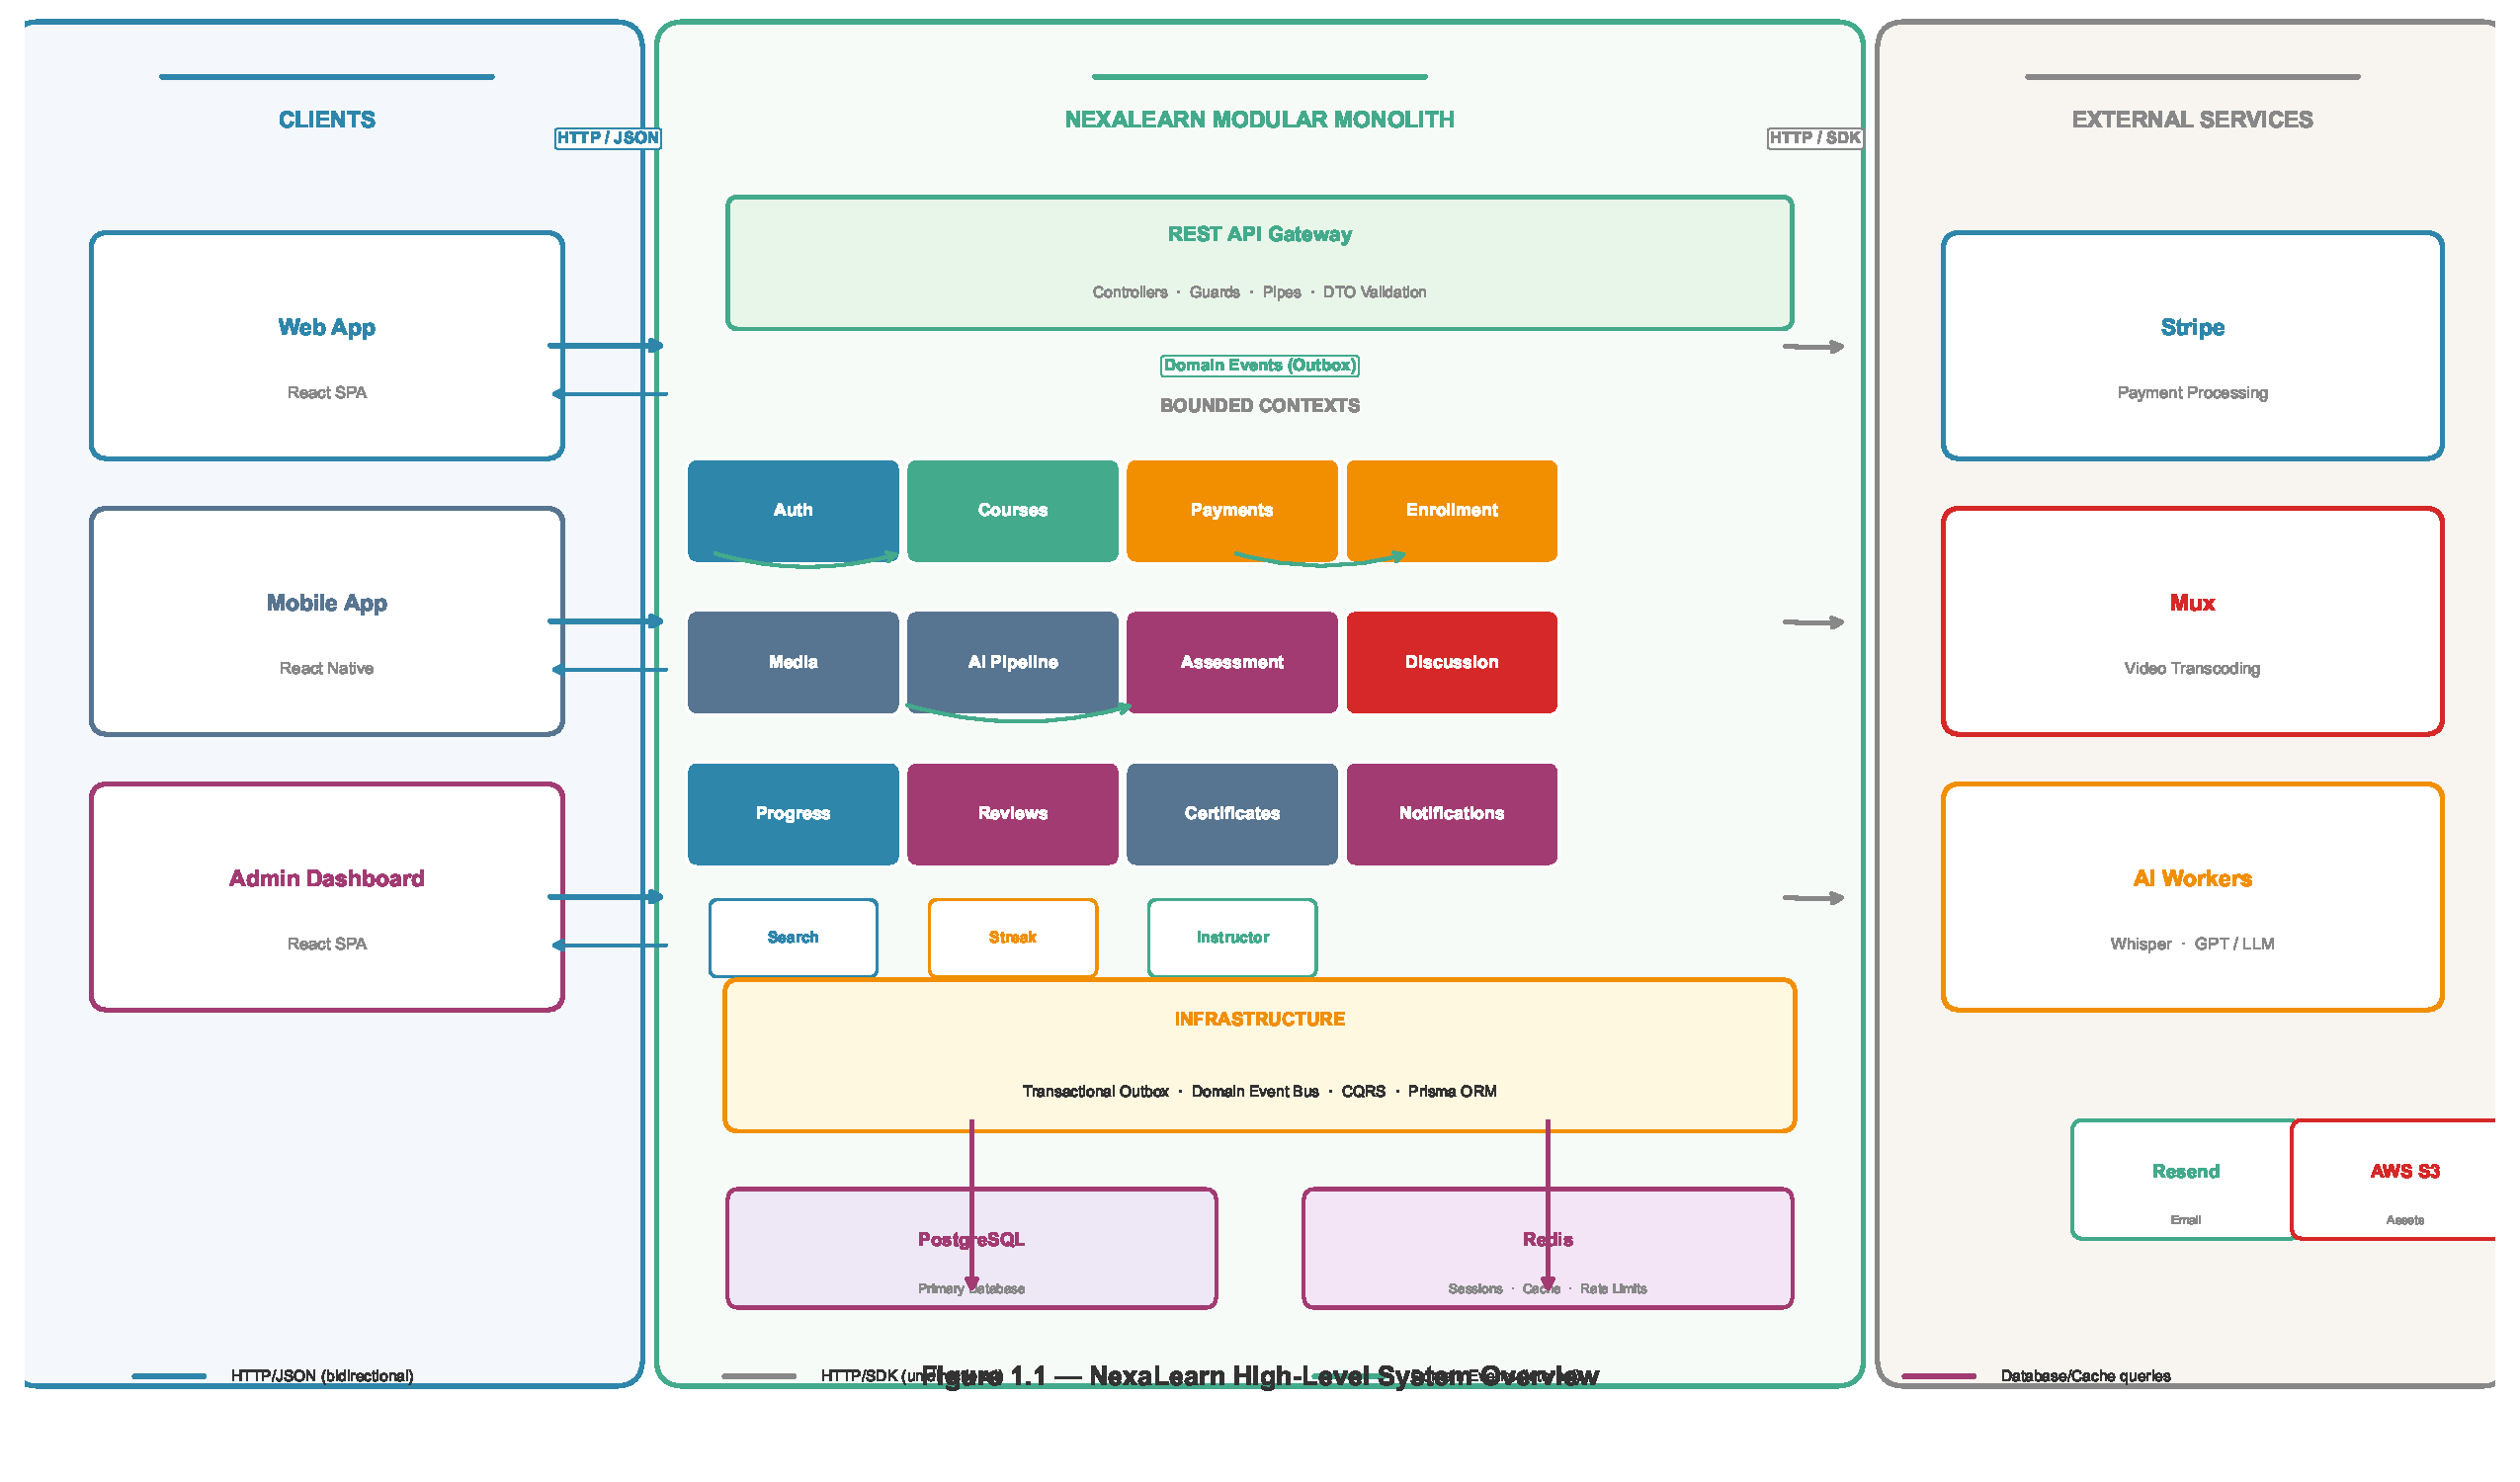
\includegraphics[width=\textwidth]{images/system_overview.pdf}
  \caption{NexaLearn High-Level System Overview}
  \label{fig:system-overview}
\end{figure}

Figure~\ref{fig:system-overview} illustrates NexaLearn's placement within the broader ecosystem: client applications (web, mobile, admin dashboards) consume a REST API exposed by a modular monolith; internal modules communicate via domain events persisted to a transactional outbox; external integrations include Stripe (payments), Mux (video), AWS S3 (supplementary assets), Resend or equivalent (transactional email), Redis (sessions, cache, rate limits), and external AI workers (Whisper transcription, LLM question generation). The diagram reflects a deliberate \textit{modular monolith} stance---operational simplicity with internal seams ready for future extraction if scale demands.

\subsection{Justification of the NexaLearn Approach}
\label{subsec:justification}

The justification for undertaking NexaLearn as a graduation project rests on four pillars aligned with both academic evaluation criteria and industry practice.

\textbf{Reference implementation gap.} No widely cited open codebase demonstrates end-to-end e-learning backend composition with DDD, Clean Architecture, transactional outbox, Stripe/Mux/AI integrations, and Testcontainers-backed integration tests in TypeScript. NexaLearn fills this gap for students, instructors evaluating the project, and future teams seeking a reproducible starting point.

\textbf{Production-grade reliability as a learning objective.} Computer Engineering graduates must understand patterns that distinguish demo-quality software from operable systems: idempotency, exactly-once side effects, webhook signature verification, optimistic locking, and structured audit logging. NexaLearn embeds these patterns in working code with tests, not merely in slides.

\textbf{Modular monolith pragmatism.} Microservice decomposition introduces distributed tracing, service mesh, and cross-service transaction complexity disproportionate to a graduation project timeline. A well-structured modular monolith delivers clear module boundaries and event-driven decoupling while remaining deployable via Docker Compose---satisfying the faculty requirement that interested readers could replicate the system without a Kubernetes cluster.

\textbf{Capstone coherence for Cairo University.} The project integrates database design, API engineering, security, cloud service integration, AI pipeline orchestration, and software architecture---competencies expected of Computer Engineering graduates. The resulting artefact is defensible in viva examination, extensible by subsequent cohorts, and portfolio-worthy for industry recruitment.

In summary, NexaLearn is motivated by market scale, architectural fragmentation in existing alternatives, the non-trivial reliability demands of async e-learning workflows, and the emerging necessity of AI-augmented content pipelines---and justified as a rigorous, open reference that future engineers can study, deploy, and improve.
